\begin{figure}
  \centering
  %\subfloat[\textbf{1 Thread.}]{\includegraphics[width=\linewidth]{graphs/Latency1Thread.pdf}}
  %\qquad
  %\subfloat[\textbf{8 Threads.}]{\includegraphics[width=\linewidth]{graphs/Latency8Threads.pdf}}
  \includegraphics[width=.55\linewidth]{PersistencyEval/Latency1Thread.pdf}
  \caption{\textbf{Persistency Model Performance vs Persist Latency.} \emph{Copy While Locked}, 1 thread.  At low persist latency all persistency models compute-bound (horizontal line formed at top).  As persist latency increases each persistency model becomes persist-bound and thereafter throughput degrades.  Relaxed persistency models are resilient to large persist latency.}
  \label{fig::RelaxedPerformance}
\end{figure}
